\chapter{系统设计}
\label{chap:SystemDesign}


\section{系统内核}

\subsection{内存管理}

\subsection{进程通信}

\section{异步I/O}

\subsection{ring\_scheduler}

\subsection{异步}

\section{模块设计}

\subsection{静态模块}

在静态模块的设计中,系统模块设计应当遵循以下原则:

\begin{enumerate}
    \item 最小正交化的模块
    \item 树状依赖和空间隔离
\end{enumerate}

\subsubsection{最小正交的模块}


\begin{figure}[htb]
    \figureCapSet
    \centering
    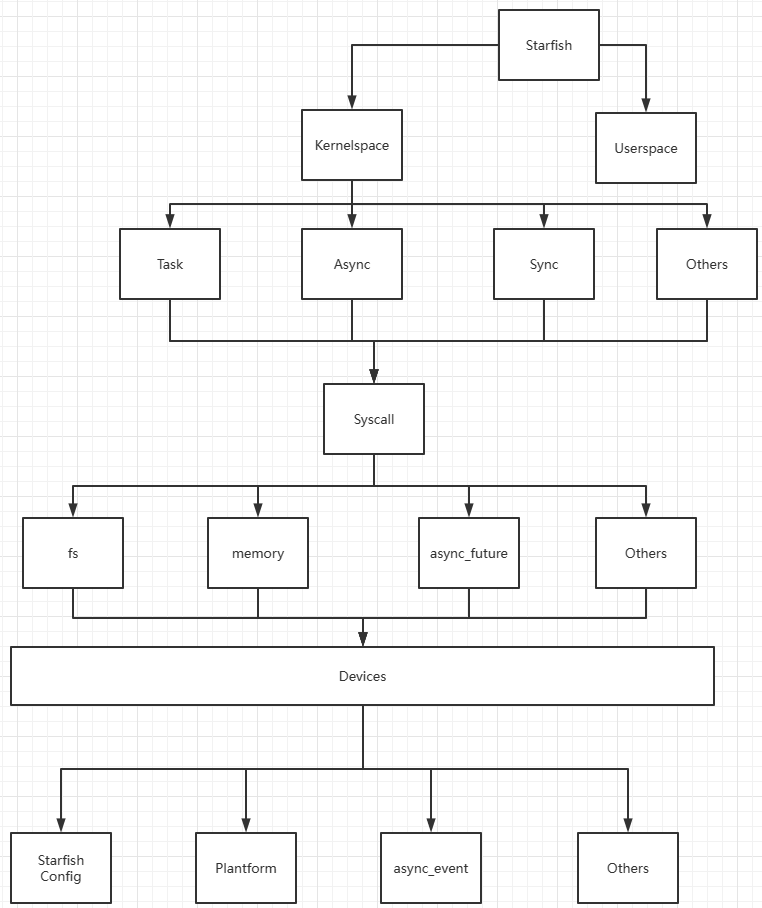
\includegraphics[width=.8\linewidth]{figure/c3/starfishstructure.png}
    \caption{Starfish 的静态模块分解图}
    \label{figure:c3starfishstructure}
\end{figure}

参考\autoref{figure:c3starfishstructure},这是最开始设计的内核模块的静态的拆分图。为了方便描述,每一层定义为抽象层级,处在最底层的其抽象层级为0,层级越低抽象的能力越小,反之则越大。而每一层的节点可以定义为抽象因子。例如,Starfish Config为0层的抽象因子,其寓意为在该层级的最小正交因子(即在当前的抽象下,该因子为最小的不可再分割的正交参考)。

正交,顾名思义就是将一个复杂的“合力”,通过相应的参考系,进行有序分解,形成一个可以通过参考系中的相应因子描述的矢量,例如 $\boldsymbol {v}=(a, b)$, 则可以准确表述矢量$\boldsymbol {v}$在直角坐标系中的空间表示。同理$\boldsymbol{E}=(L, F)$则表述模块在层级间的空间表述,其中$\boldsymbol{E}$表示评估因子,L表示抽象层级,F表示抽象因子。由此可以总结出两组概念:最小正交化和严格最小正交化。

\begin{enumerate}
    \item 最小正交化: 当$L=0$时,即抽象层级为0,即模块不可再分的情况下, $\boldsymbol{E}$为最小正交化的评估因子,此时模块分解为最小正交化。
    \item 严格最小正交化: 在满足最小正交化的前提下, 有$F = {F_{0}, F_{1}, \cdots, F_{n}}$,其中$0 = {F_{0} \cap F_{1} \cap \cdots \cap F_{n}}$, 此时, $\boldsymbol{E}$为严格正交化的评估因子,此时模块分解为严格最小正交化。
\end{enumerate}

当$\boldsymbol{E}$为严格正交化时,则可以说模块分解达到了一个最优的状态,此时所有的$L=0$级的模块之间不存在互相干扰的情况,彼此之间的联系,仅仅通过语言编程者之间的API约束,如此的好处可以使得模块之间的耦合程度变低,相互之间可以独立进行开发,同时如果他人的内核也遵循了相应的API约束,则该模块可以达到共享的目的。


\subsubsection{树状依赖和空间隔离}


通过\autoref{figure:c3starfishstructure}的观察,可以发现模块的分解和组合,其静态的模块将会形成一种树状的结果,此时L(即抽象层级)之间是存在“方向”的,即当存在$L_{i} < L_{j} (i < j)$时, $L_{j}$必然是由部分$L_{i}$组成,而必不可能存在上下互换的生成形式,如若L的层级方向出现错误,则$\boldsymbol{E}$将无法做出评估,其模块拆解也必然是错误的。由此,一个良好的模块分解必然会形成一个层次分明的树状依赖。

当L一定, $F = {F_{0}, F_{1}, \cdots, F_{n}}$时, 若有$0 = {F_{0} \cap F_{1} \cap \cdots \cap F_{n}}$,此时的$\boldsymbol{E}$可以达到最优解,即优化评估因子,记作$\boldsymbol{OE}$,特别地当 $L = 0$时,若形成$\boldsymbol{OE}$,即$F$达到分解地最优解,则此时就可以称为严格最小正交化。

其中$\boldsymbol{OE}$的意义是,层级间的依赖被解除,模块是独立,没有相互干扰, 可以达到层级空间间的空间隔离。同样以此可以逆向评估底层模块的$\boldsymbol{E}$特性, 通过数学归纳法,我们可以显而易见的得出当$L_{i} < L_{j} (i < j)$, 若$L_{j}$达到了$\boldsymbol{OE}$,则$L_{i}$也应当是$\boldsymbol{OE}$的。

\subsection{动态模块}

在动态模块的设计中,系统的模块设计应当遵循以下三个原则: \begin{enumerate}
    \item 需要获取所有模块的运行时的持久边界
    \item 最大限度地发挥语言(Rust)和编译器的作用
    \item 最小化模块之间的状态溢出
\end{enumerate}

\subsubsection{需要获取所有模块的运行时的持久边界}

系统内核中的模块组件具有明确定义的边界(严格化的正交模块),并在整个运行时保持不变: 在实现时,系统模块组件以Rust独立的Crate的形式存在;在编译时,系统模块组件以一组加载的内存区域的形式存在;在运行时,系统模块组件以一组加载内存区域的形式存在,内存区域具有每部分的边界和依赖元数据。

上述的设计原则每一个内核的系统模块组件都需要遵循。运行时,可以显示识别系统模块组件的边界是系统内核中组件隔离和状态管理的基础。

在运行时,系统内核根据需要将所有系统模块组件加载并链接到系统中。简而言之,这需要找到并解析系统模块组件对象,将其部分加载到内存中,解析其依赖,根据依赖树,以写入连接器重定位条目,根据需要递归加载任何丢失的系统模块组件,并向符号映射添加新的公共符号。基于此可以为内核进化和故障恢复提供理论基础。加载的系统模块组件集定义了一个系统模块组件空间,一个包含所有系统模块组件公共符号的真正的名称空间,用于快速解析单元格之间的依赖关系。每个加载的系统模块组件节点跟踪其组成部分和存储区域包含它们。每个系统模块组件中的部分对应于其Crate的目标文件中的部分,例如,可执行文件、只读数据和读写数据部分。每个加载的分段节点跟踪其大小、在存储器中的位置以及双向依赖性(输入和输出);额外的元数据用于加速系统模块组件交换和其他系统功能。

系统模块组件边界的持久性降低了复杂性: 系统内核的持久性系统模块组件边界在其存在的所有阶段提供了一致的系统结构抽象。这将会降低了开发者对系统的理想模型的复杂性,并简化了故障恢复和演化逻辑,因为系统内核可以在运行时从相同的面向系统模块组件的角度自省和管理它自己的代码。从顶层应用程序和库到核心内核组件的一切都可以作为系统模块组件来观察。这使得系统内核能够

\begin{itemize}
	\item 实现统一适用于任何单元的单一机制,即模块交换,以及
	\item 以安全的方式从多个系统层(例如,应用和内核组件)联合进化模块。
\end{itemize}

\subsubsection{最大限度地发挥语言(Rust)和编译器的作用}
通过使编译器能够最大限度地检查安全性和正确性不变量来最大限度发挥语言的力量。

将系统内核的执行环境与该语言的运行时模型相匹配,并在Rust等现代语言提供的强大的静态类型系统中实现操作系统概念。这将编译器检查的不变量(例如,没有悬空引用)扩展到了所有类型的资源,而不仅仅是语言中内置的那些。

依赖语言设计有两个主要好处:

\begin{itemize}
    \item 首先,它使编译器能够接管资源管理职责,减少了操作系统必须维护的状态,从而减少了状态溢出并加强了隔离。
    \item 它使编译器能够在理解代码行为的过程中应用安全检查,从应用程序到核心内核组件实现端到端安全,并将语义运行时错误转化为编译时错误。
\end{itemize}

相比之下,传统的非语言方法依赖于硬件保护和运行时检查来维护安全性、隔离性和正确性的不变量。这些特性对编译器是透明的,需要不安全的代码。甚至现有的安全语言操作系统。在语言级别的安全代码和底层的不安全核心之间有一个缺口,后者将语言所需的抽象实现为一个黑盒。

\subsubsection{最小化模块之间的状态溢出}

由于系统内核的组件结构是模块化的,因此状态溢出只能发生在跨越模块边界并导致接收单元状态改变的交互(例如,函数调用)中。
